\chapter{Fonctions}

\section{Ensembles de nombres} : Réels $\mathbb{R}$, Rationnels $\mathbb{Q} = \cfrac{a}{b}$ avec a et b entiers naturels $\mathbb{N}$, entiers $\mathbb{Z}$ = $\{-3, -2, ..., 1\}$, nombres complexes $\mathbb{C}$.
\section{Intervalle} : [a, b] avec a, b réels compris dans l'intervale, dit fermé, $a < b$, ]a, b[ avec a, b non compris dans l'intervale dit ouvert $\rightarrow$ Intervalle bornés
$\mathbb{R} = ]-\infty; +\infty[ \mathbb{R}^* = ]-\infty; 0[ \cup ]0; +\infty[ \mathbb{R}^+ = [0; +\infty[ \mathbb{R}^- = ]-\infty; 0]$

\section{Fonctions}
\ul{Exemple} : sinus : $\sin : \mathbb{R}$ (domaine de definitions, sources, ensemble de depart) $\rightarrow \mathbb{R}$ ou$ [-1, 1]$ (domaine de valeurs, image, but, ensemble d'arrivee)

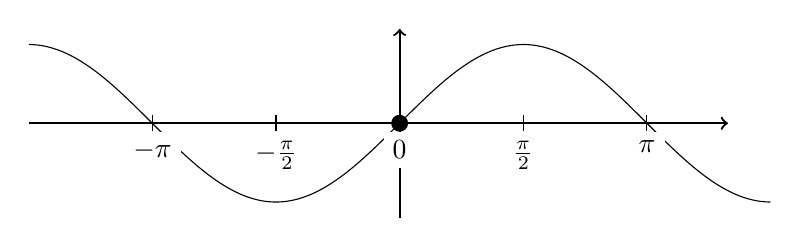
\begin{tikzpicture}

\draw[->, thick, black] (0, -1.2) -- (0, 1.2);
\draw[->, thick] (-4.71, 0) -- (4.17, 0);
\draw[domain=-4.71:4.71, samples=500] plot (\x, {sin(\x r)});
\draw[fill=black] (0, 0) circle (0.1);
\foreach \x/\text in {
	-3.14/$-\pi$, 
	-1.57/$-\frac{\pi}{2}$,
	0/0, 
	1.57/$\frac{\pi}{2}$,
	3.14/$\pi$}
	\draw[] (\x, 0.1) -- (\x, -0.1) node[below, fill=white] {\text};

\end{tikzpicture}

\paragraph{Définitions} Soit E, F 2 ensemble de R. Une fonction f est procédé pour associer à tout élément de R un unique élément de F
Le graph de F "vit" dans $\mathbb{R}^2 = \mathbb{R}*\mathbb{R}$
\paragraph{Définitions} : Soit E et F 2 ensembles, on définit leur \ul{produit cartesien} :  comme l'ensemble dont les éléments sont les couples $(x, y)$ avec x "vit" dans E et y dans F. ~\\
ExF = \{(x, y), $x \in E, y \in F$\}
\paragraph{Définitions} : Le \ul{graphe} de f :$ E \rightarrow F$ est un sous ensemble de $E*F$ donné par ~\\

$\begin{array} {r l}
E*F = & \{(x, y), x \in E, y =f(x)\}\\
E*F = & \{x:\rightarrow f(x) = y\}
\end{array}$

\paragraph{Exemples} cosinus : $\cos : \mathbb{R} \rightarrow [-1, 1]$ ~\\

\begin{wrapfigure}{r}{0pt}
	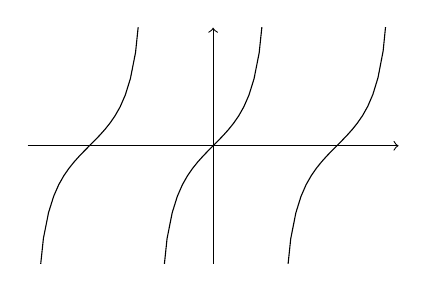
\begin{tikzpicture}[scale=0.5]

\clip (4.71, 3) -- (4.71, -3) -- (-4.71, -3) -- (-4.71, 3) --cycle;

\draw[->] (-4.71, 0) -- (4.71, 0);
\draw[->] (0,-3) -- (0, 3);

\draw[domain=-1.56:1.56] plot(\x, {tan(\x r)});
\draw[domain=-4.70:-1.58] plot(\x, {tan(\x r)});
\draw[domain=1.58:4.71] plot(\x, {tan(\x r)});

\end{tikzpicture}
\end{wrapfigure}
tangeante $\tan : \mathbb{R} \backslash\{\pi/2 + k*\pi,$ k appartient a Z\}$ \rightarrow$ $]-\infty, +\infty[$


\begin{tikzpicture}
	\draw[->] (-2.2, 0) -- (2.2, 0);
	\draw[->] (0,-2.2) -- (0, 2.2);

	\draw[] (0, 0) circle (2);
	\draw[] (0, 0) -- (30:2) coordinate (A);

	\draw[->, blue] (1, 0) arc (0:30:1);
	\getxy{\xa}{\ya}{A}
	\draw[dashed, fill=white] (A) -- (\xa, 0) node [below, blue] {$\cos(x)$};
	\draw[dashed] (A) -- (0, \ya) node [left, blue] {$\sin(x)$};

	\path[name path=line 1] (0, 0) -- (30:4);
	\path[name path=line 2] (2, 5) -- (2, -5);
	\draw[name intersections={of=line 1 and line 2}, red] (intersection-1) coordinate (T);
	\getxy{\xt}{\yt}{T}
	\draw[dashed] (T) -- (\xt, 0) node [midway, right] {$\tan(x)$};
	\draw[dashed] (0, 0) -- (T);
\end{tikzpicture}

\begin{math}
\tan(x) = \frac{\sin(x)}{\cos(x)}
\newline
\mathbb{R} \rightarrow \mathbb{R}
x \rightarrow x^n, n \in N
\newline
n = 0 : x \rightarrow 1
\newline
n = 1 :
x \rightarrow x
\newline
n = 2 : 
x \rightarrow x^2
\newline
n = 3 :
x \rightarrow x^3
\end{math}

~\\
~\\
~\\
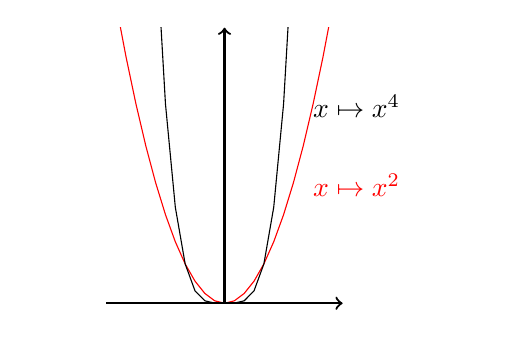
\begin{tikzpicture}[scale=0.5]
	\clip (7, 7) rectangle (-5, -0.5);
	\draw[domain=-3:3, red] plot(\x, {\x * \x});
	\node at (2, 3) [red, right] {$x \mapsto x^2$};
	\draw[domain=-3:3] plot(\x, {\x * \x * \x * \x});
	\node at (2, 5) [black, right] {$x \mapsto x^4$};
	\draw[->, thick] (-3, 0) -- (3, 0);
	\draw[->, thick] (0, 0) -- (0, 7);
\end{tikzpicture}
Remarque : les fonctions sont plus étroites. Schéma typique pour $n >0$ et n pair.

\paragraph{Définitions} Soit $f:E \rightarrow R$ une fonction, avec E symétrique par rapport à 0.
\begin{itemize}
	\item f est dite \ul{paire} si : $\forall x \in E, f(-x) = f(x)$
	\item f est \ul{impaire} si : $\forall x \in E, f(x) = - f(-x)$ Remarque : si f est impaire $\rightarrow f(0) = 0$ . En effet, 
		\begin{eqnarray}
			f(-0) & = & f(0) \\
			f(0) & = & -f(0) \\
			2*f(0) & = & 0
		\end{eqnarray}
\end{itemize}

Exemple : fonctions paire : cosinus, $x^{2p}$ avec p appartient à N ~\\
impaires sinus, tangeante, $x^{2p+1}$ avec p appartient à N

\section{monotonie} Soit $f:E \rightarrow \mathbb{R}$

\begin{itemize}
	\item f est \ul{croissante} si $a < b,$ alors $f(a) \leq f(b)$ avec $a, b \in \mathbb{R}$
	\item f est \ul{strictement croissante} si $a < b$, alors $f(a) < f(b)$ avec $a, b \in \mathbb{R}$
	\item f est \ul{decroissant} si $ \forall \{a, b\} \in \mathbb{R}$ avec $a < b,$ alors $f(a) \geq f(b)$
	\item f est \ul{decroissant} si $ \forall \{a, b\} \in \mathbb{R}$ avec $a < b,$ alors $f(a) > f(b)$
\end{itemize}

\paragraph{Exemple} $f: \mathbb{R}^* \rightarrow \mathbb{R}^*
x \rightarrow \frac{1}{x}$

\begin{tikzpicture}
	\clip (-5, 5) -- (-5, -5) -- (5, -5) -- (5, 5) -- (-5, 5);
	\draw[->] (-5, 0) -- (5, 0);
	\draw[->] (0, -5) -- (0, 5);
	\draw[domain=-5:-0.01] plot(\x, {1/(\x)});
	\draw[domain=0.01:5] plot(\x, {1/(\x)}) node [thick, xshift=-7cm, above] {$y=\frac{1}{x}$};
\end{tikzpicture}

décroissante sur $]-\infty, 0[ et ]0, +\infty[$ mais pas sur $]-\infty, 0[ \cup ]0, +\infty[$
par exemple, $-1 \leq 1 \text{ et } \frac{1}{-1} \leq \frac{1}{1}$

\paragraph{Définition} Soit $f:E \rightarrow F$ et A un sous ensemble de E.
On appelle \ul{restriction} de f a A, note $f_{|A}$. La fonction $f_{|A} : A \rightarrow F$ definie par $f_{A}(x) = f(x) \forall x \in A$ ~\\
Soit $f:E \rightarrow F$ et E', F' des sous ensembles de R, avec $E \subset E',F \subset F' . $ ~\\
La fonction $ g : E' \rightarrow F'$ est un \ul{prolongement} de f si $g_{|E} = F(x)$ c'est à dire $\forall x \in E, g(x) = f(x)$

\paragraph{Exemple} logarithme népérien $ln : ]0, +\infty[ \rightarrow \mathbb{R}$
	~\\
	$x \rightarrow ln(x)$
	~\\
	$ln(a) + ln(b) = ln(a*b)$ avec $\forall (a, b) \in (R^{*+})^2$


\section{Opérations sur les fonctions}
Soit $f, g : E \rightarrow \mathbb{R}$. On peut définir :

\begin{itemize}
	\item La fonction somme $f+g$ par $f+g : E \rightarrow \mathbb{R} \text{ }
		x\rightarrow(f+g)(x) = f(x)+g(x)$
	\item La fonction produit $f*g$ par $f*g : E \rightarrow \mathbb{R} \text{ }
		x\rightarrow(f*g)(x) = f(x) \dot g(x)$
\end{itemize}

\section{Image (direct) d'une fonction composé (composition)}
\paragraph{Définitions} : $f:E \rightarrow F$. \ul{L'image} de f notée $im(f)$ c'est l'ensemble $\{y \in F$ tel que il existe $x \in E$ tel que $f(x) = y\}$ aussi noté $f(E)$

\paragraph{Définition} $f:E \rightarrow F$ et $g:E' \rightarrow F'$
Si l'image de $g \subset E$, on peut définir la fonction composé $f o g : E' \rightarrow F$ 
~\\
$x \mapsto f o g (x) = f(g(x))$

\section{Image réciproque} 
\paragraph{Définition} Soit $f:E \rightarrow F$, et $B \subset F$ L'image réciproque de B par f est l'ensemble  $f^{-1}(B) = \{x \in E$ tel que $f(x) \in B\}$

$f^{-1}([-1, 1]) = [a, b]$
